\chapter{Le fondement des années}\label{ch:fondement}

Une année de classement n’est pas une date établie. Ce chapitre rapporte chaque année à ce qui la fonde dans le texte transmis, en distinguant les lettres lues, les lettres restituées par l’éditeur et les données qui proviennent de la seule base de données.

\section{Année de la base, année du texte, année de classement}

La base de travail distingue, pour chaque notice, l’année fournie par l’EDCS, l’année déduite du texte lorsque les consuls nommés la déterminent, et l’année retenue pour le classement, accompagnée d’une justification. L’année de classement est celle de la base, sauf lorsque le texte la contredit de manière univoque. Sept notices sont dans ce cas (tableau~\ref{tab:correctionsbase}) ; l’année de la base reste consultable dans les données. Pour quatre d’entre elles, la confrontation avec l’EDB a fait apparaître une autre lecture possible : la correction est maintenue, mais la datation est déclarée contestée.

\begin{table}[tbp]\centering\small
\caption{Années de la base corrigées d’après le texte.}\label{tab:correctionsbase}
\begin{tabularx}{\linewidth}{@{}r r r X@{}}\toprule
N° & Base & Classement & Justification et état actuel\\\midrule
12 & 345 & 352 & Deux formules consulaires ; \emph{-aulo conss.} est lu et Paulus n’est consul qu’en 352 ; \emph{Amantio et Albino} (345) date un événement antérieur non précisé.\\
206 & 377 & 370 & \emph{Valentiniano III et Valente Augg.} ne convient qu’à 370 ; l’EDB date aussi de 377, vraisemblablement par erreur de saisie.\\
278 & 385 & 383 & \emph{Merobaude II et Saturnino} = 383 ; l’EDB date de 385, mais date de 383 une fiche voisine du même consulat.\\
311 & 389 & 388 & \emph{Maximo cons(ule)} : consulat de Magnus Maximus (388). L’EDB date de 389 : contestée.\\
314 & 389 & 390 & Formule \emph{Valentiniano Aug. IIII et Neoterio} (390), entièrement restituée sauf \emph{d(omino) n(ostro) V}. Contestée.\\
328 & 390 & 381 & Seul \emph{…terio} est lu : Eucherius (381) ou Neoterius (390). Contestée.\\
434 & 399 & 397 & \emph{p(ost) cons(ulatum) Arcadi I[II]I} = 397 ; l’EDB date de 399.\\\bottomrule
\end{tabularx}
\end{table}

Deux autres cas relèvent du calcul interne. Au \nnum{19}, Lea est morte sous Amantius et Albinus (345) ; l’année 347 de la base paraît déduite d’une indication « il y a deux ans » que l’EDCS restitue et que l’EDB ne retient pas : le texte est daté au plus tôt de 345. Au \nnum{55}, la discordance apparente se résout par le calcul : le défunt est né sous Acindynus et Proculus (340), le 21 juin ; 19 ans, 3 mois et 6 jours plus tard, on parvient au 27 septembre 359, qui est exactement le 5\textsuperscript{e} jour avant les calendes d’octobre gravé comme date de déposition.

\section{Lire, restituer : quatre niveaux pour le nom consulaire}

L’identification d’un collège consulaire ne dit pas, à elle seule, ce qui en est lu. La formule \emph{[Acin]dino et Procu[lo conss(ulibus)]} permet d’identifier l’année 340, mais les deux noms n’y sont conservés qu’en partie. Pour chaque texte à datation directe, l’état de lecture de chaque nom consulaire a donc été relevé sur la transcription, puis classé selon le meilleur nom :

\begin{description}[style=nextline,leftmargin=1.5em,font=\normalfont\scshape]
\item[A — nom lu] au moins un nom consulaire est entièrement lu ;
\item[B — lecture partielle] au moins trois lettres gravées d’un nom sont lues, le reste étant restitué ;
\item[C — initiales] les noms sont réduits à des initiales (\emph{M(amertino) et N(evitta)}, \nnum{70}) ;
\item[R — consulat restitué] aucun nom n’atteint le niveau B : l’année repose sur une restitution de l’éditeur, guidée par des lettres isolées, une itération ou le contexte.
\end{description}

Dans l’ensemble C, l’année de \st{datLu} textes repose sur un nom consulaire lu, celle de \st{datPartiel} sur une lecture partielle, celle de \st{datInit} sur des initiales et celle de \st{datRest} sur un consulat restitué (tableau~\ref{tab:datation}, figure~\ref{fig:annees}). Le niveau R ne signifie pas que l’année est fausse : la restitution est souvent contrainte par une itération ou une titulature. Il signifie qu’elle ne peut pas servir de jalon indépendant pour dater d’autres textes.

% généré par scripts/04_generated.py
\begin{table}[tbp]\centering\small\caption{Fondement de l’année dans l’ensemble C (n = 465). Les listes de plus de quarante notices sont données dans la chronique (chapitre~\ref{ch:chronique}).}\label{tab:datation}
\begin{tabular}{@{}p{0.36\linewidth} r p{0.5\linewidth}@{}}\toprule Fondement & Textes & Notices\\\midrule
Directe : nom consulaire lu & 330 & {\footnotesize —} \\
Directe : lecture partielle d’un nom consulaire & 96 & {\footnotesize —} \\
Directe : initiales consulaires & 2 & {\footnotesize 48, 70} \\
Directe : consulat restitué & 21 & {\footnotesize 52, 129, 137, 138, 161, 203, 219, 222, 256, 290, 314, 384, 393, 415, 426, 432, 438, 452, 455, 465, 468} \\
Formule transmise par l’EDB (lue) & 4 & {\footnotesize 84, 214, 268, 388} \\
Formule transmise par l’EDB (lue, itération restituée) & 1 & {\footnotesize 445} \\
Formule transmise par l’EDB (partiellement restituée) & 3 & {\footnotesize 51, 180, 447} \\
Conjecturale & 4 & {\footnotesize 123, 326, 435, 457} \\
Indirecte & 4 & {\footnotesize 36, 267, 348, 349} \\
\bottomrule\end{tabular}\end{table}


\begin{figure}[tbp]\centering
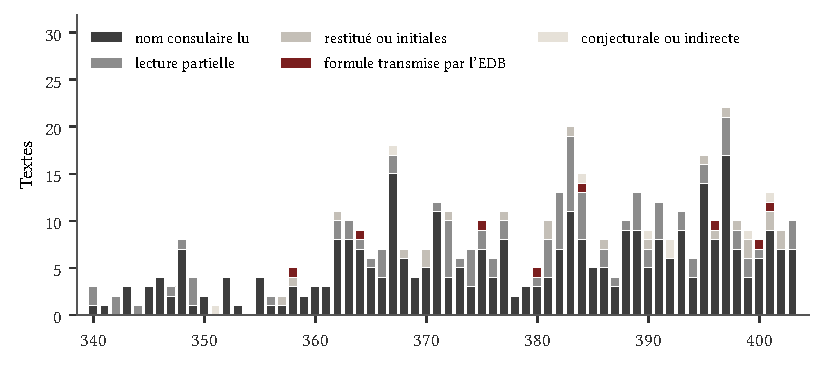
\includegraphics[width=\linewidth]{figures/fig_annees.pdf}
\caption{Textes de l’ensemble C par année de classement et par fondement de l’année.}\label{fig:annees}
\end{figure}

\section{Huit formules transmises par la seule EDB}

Pour seize notices du catalogue initial, le texte EDCS ne conservait aucun élément consulaire, et l’année provenait de la base. La confrontation avec l’EDB modifie ce constat pour huit d’entre elles, dont la formule de date est transmise par la seconde base :

\begin{itemize}
\item formule lue : \nnums{84} (Jovien et Varronianus, 364), 214 (Gratien V et Théodose, 380), 268 (Richomer et Clearchus, 384), 388 (Arcadius IV et Honorius III, 396) ;
\item formule lue, itération restituée : \nnum{445} (\emph{Stellici v(iri) c(larissimi) [iterum?]}, 400, ou 405 si \emph{iterum} est retenu) ;
\item formule partiellement restituée : \nnums{51} (Cerealis, 358), 180 (post-consulat d’Equitius, 375), 447 (Fravitta, 401).
\end{itemize}

Quatre autres notices reçoivent de l’EDB une restitution conjecturale (\nnums{123}, 326, 435 et 457). Au \nnum{123}, les deux lectures sont incompatibles : là où l’EDB restitue \emph{[Lupicin?]o et ⟨I⟩ovi[no]}, l’EDCS lit \emph{[- - -]o et o⸢b⸣i[it]}, « et mourut ». Ces quatre textes sont classés « conjecturaux ». Restent quatre textes dont l’année provient de la seule base, sans formule consulaire dans aucun témoin : \nnums{36} (datation prosopographique), 267 (fragment), 348 (épitaphe grecque d’Alexandros) et 349 (épitaphe de Leoparda, dont le jour de la semaine et l’âge de la lune sont compatibles avec 392 ; chapitre~\ref{ch:calendrier}).

\section{Faux consuls}

L’identification automatique des consuls, qui rapproche les noms du texte d’une liste de consuls, a produit des erreurs de rôle : \st{nFauxConsuls} noms, dans \st{nFauxConsulsNotices} notices, désignent en réalité un défunt, un dédicant, une personne citée ou un fonctionnaire. Ainsi, au \nnum{68}, \emph{Eutyches pater fecit} nomme le père qui commémore, non le consul Eutychianus de 398 ; au \nnum{55}, \emph{Marcellinus} est le défunt ; au \nnum{321}, \emph{Fl(avius) Filippus} est le responsable des travaux de la colonne de Saint-Paul et \emph{Paul(us)} l’apôtre ; au \nnum{462}, \emph{Saturninus} est le défunt. Aucune de ces erreurs ne modifie l’année de classement, qui repose dans tous les cas sur l’autre consul ou sur le collège complet. Les rôles corrects sont donnés dans chaque notice (rubrique Chronologie) et dans l’index des consuls.

\section{Datations contestées et réserves}

Dix datations sont contestées : deux lectures publiées, ou deux restitutions également possibles, conduisent à deux années différentes. Cinq autres font l’objet d’une réserve : la formule transmise ne concorde pas entièrement avec le collège de l’année de classement. Deux divergences, enfin, sont vraisemblablement des erreurs de saisie de l’EDB. Le tableau~\ref{tab:contestees} donne les motifs. Dans tous les cas, l’année de classement est conservée : aucune année n’est modifiée par vraisemblance.

% généré par scripts/04_generated.py
\begin{longtable}{@{}r r l p{0.6\linewidth}@{}}\caption{Datations contestées, réserves et divergences attribuées à l’EDB. L’année de classement est conservée dans tous les cas.}\label{tab:contestees}\\\toprule N° & Année & Statut & Motif\\\midrule\endfirsthead\toprule N° & Année & Statut & Motif\\\midrule\endhead\bottomrule\endfoot
40 & 353 & contestée & {\footnotesize Magnence III et Décence II (353) selon la lecture retenue ; l’EDB, citant CLRE p. 636, date de 352 en supposant une erreur du lapicide.} \\
52 & 358 & contestée & {\footnotesize Da[tiano] (358) selon Silvagni ; la CLRE (p. 631, citée par l’EDB) rappelle que Dalmatius, consul en 333, commence aussi par DA. Si 333, la notice sort du corpus.} \\
141 & 370 & contestée & {\footnotesize Valentinien III : Valentinien Ier (370) ou Valentinien II (387) ; la CLRE (p. 644, citée par l’EDB) note « Year doubtful: 387 possible ».} \\
165 & 372 & contestée & {\footnotesize L’année 372 repose sur la seule séquence « dest », interprétée par Ferrua comme [Mo]dest[o] ; l’EDB date « 300-399 ».} \\
206 & 370 & EDB fautive & {\footnotesize L’EDB date de 377 ; la formule Valentiniano III et Valente Augg. ne convient qu’à 370 : erreur probable de saisie de l’EDB.} \\
220 & 381 & contestée & {\footnotesize Seul …erio est lu ; l’EDB signale d’autres restitutions possibles (Val]erio, Gal]erio, Neot]erio, Ast]erio) : 381 ou 390.} \\
278 & 383 & EDB fautive & {\footnotesize L’EDB date de 385 ; Merobaude II et Saturnino = 383, et la fiche voisine EDB8750 (même consulat) est datée de 383 : incohérence interne probable de l’EDB.} \\
311 & 388 & contestée & {\footnotesize Maximo cons(ule) : consulat de Magnus Maximus (388) ; l’EDB date de 389 et signale une transcription différente de l’ICVR.} \\
314 & 390 & contestée & {\footnotesize Second texte du monument ICUR IV 11117 : seul d(omino) n(ostro) V[…] est lu ; 390 est une restitution partagée par l’EDCS et l’EDB, que la note de l’EDB juge contradictoire avec l’ordre des décès.} \\
328 & 381 & contestée & {\footnotesize Seul …terio est lu : Eucherio (381) ou Neoterio (390).} \\
395 & 396 & réserve & {\footnotesize Itération d’Honorius (IIII transmis) à confronter au collège de 396 (Arcadius IV et Honorius III).} \\
411 & 397 & réserve & {\footnotesize Collège Caesarius et Maximus ; les fastes donnent pour 397 Caesarius et Atticus.} \\
428 & 398 & réserve & {\footnotesize Post-consulat d’Honorius IV et Eutychianus (399 ?) ou consulat (398) ; le jour de la semaine (samedi) convient au 18 décembre 398.} \\
431 & 399 & contestée & {\footnotesize La CLRE (p. 661, citée par l’EDB) attribue le texte à 398 ; 399 suppose un post restitué que l’EDB juge trop long.} \\
434 & 397 & contestée & {\footnotesize Post-consulat d’Arcadius IV : 397 ; l’EDB date de 399.} \\
444 & 400 & réserve & {\footnotesize Itération [iter(um)] de Stilichon restituée ; compatibilité avec 400 à contrôler.} \\
466 & 402 & réserve & {\footnotesize Paire Arcadius–Théodose à contrôler sur les fastes de 402.} \\
\end{longtable}


\section{Distribution chronologique}

La distribution des textes funéraires par année de classement est très inégale (figure~\ref{fig:annees}). Elle progresse nettement à partir de 360, et \st{partApres380}~\% des textes de l’ensemble C appartiennent aux années 380–403. Les périodes utilisées dans la suite du livre comptent \st{perC0} textes (340–359), \st{perC1} (360–374), \st{perC2} (375–389) et \st{perC3} (390–403). Cette progression peut traduire une diffusion de la datation consulaire dans les épitaphes chrétiennes ; elle peut aussi tenir aux hasards de la conservation et de la publication. Le corpus ne permet pas de trancher entre ces explications.
